%%%%%%%%%%%%%%%%%%%%%%%%%%%%%%%%%%%%%%%%%%%%%%%%%%%%%%%%%%%%%%%%%%%%%%%%%%%%%%%
%% Introduction                                                              %%
%%%%%%%%%%%%%%%%%%%%%%%%%%%%%%%%%%%%%%%%%%%%%%%%%%%%%%%%%%%%%%%%%%%%%%%%%%%%%%%

\chapter{Introduction}
\label{chap:intro}

The \emph{ePNK} is an Eclipse based framework and platform for developing
and integrating Petri net tools and applications. One of its core features
is that new \emph{Petri net types} can be plugged in, which does not require
any programming. A new Petri net type can be defined by providing a model
of its concepts, the so-called \emph{Petri net type definition} (\emph{PNTD}).
In addition, the ePNK allows adding new \emph{applications} on Petri nets
to the ePNK.

The ePNK builds on the concepts and models of the \emph{Petri Net Markup
Language} (\emph{PNML})
\cite{ISO-IEC:15909-2-2011,JKW00b,JKW00b,WeKi03,BCea03}.%
  \index{PNML}
Therefore, we start with a brief overview of the PNML, and then discuss
the concepts and ideas of the ePNK and its main features.

In the end of this chapter, there is some information for
different kinds of readers on what to read and on how to read this manual.

\section{Motivation}
\label{chap:motivation}

The PNML is an XML-based interchange format for all kinds of Petri nets,
which allows different tools to exchange Petri net models among each other.
One of PNML's main features is that it is generic, which means that it provides
a mechanism for defining own types of Petri nets, which are called \emph{Petri
net type definitions} (\emph{PNTD}).%
  \index{PNTD}
These Petri net type definitions define the
additional concepts of the new Petri net type, as well as the representation of
these new concepts in XML syntax. It is also possible that different
tools include \emph{tool specific information}%
  \index{Tool specific information}
to PNML documents, which is information that can be safely ignored by
other tools.

Before the ePNK, there was no tool that fully supported these ideas in such a
way that the tool would allow a developer to define and plug in new
\emph{Petri net types}%
  \index{Petri net type}
and additional tool specific extensions. And there was no
generic editor supporting all Petri net types, once they are plugged in.

The lack of such a generic tool support was the starting point for
developing the \emph{ePNK}.

\section{The Petri Net Markup Language}
\label{sec:intro:PNML}
\index{PNML|(DEF}
In order to better understand the ideas of the ePNK, we briefly discuss the
main concepts and ideas of the PNML here. For more information
on the PNML and on ISO/IEC~15909-2, we refer to \cite{Kin06,HKea09} or to
the International Standard ISO/IEC~15909-2:2011 itself
\cite{ISO-IEC:15909-2-2011}.

\subsection{The PNML core model}
\label{subsec:PNMLcoremodel}

As stated above, extensibility and genericity were two of the main
objectives behind the PNML \cite{JKW00}. This is achieved by identifying the
concepts that are common to all kinds of Petri nets in the so-called \emph{PNML
core model}.% 
  \index{PNML core model|(DEF}
The common concepts are mainly \emph{places}, \emph{transitions}%
  \index{Place|DEF}%
  \index{Transition|DEF}
and \emph{arcs}, and that these \emph{objects} can have some kind of%
  \index{Arc|DEF}%
  \index{Object (of a Petri net)|DEF}
\emph{label}.% 
  \index{Label|DEF}
The PNML core model also provides means for splitting up larger
Petri nets into \emph{pages};%
  \index{Page|DEF}
connections between nodes on
different pages can be established by \emph{reference places} or%
  \index{Reference place|DEF}
\emph{reference transitions}. And PNML defines all kinds of graphical%
  \index{Reference transition|DEF}
information that can be attached to the different elements, such as
position, size, font-type, and font-size.

Note that in graphical editors, a label would typically be shown as
an annotation attached to (or close to) the object it belongs to.  Labels
that should be shown as annotations are, therefore, called \emph{Annotations}.%
  \index{Annotation|DEF}
Some labels, however, are not supposed
to be shown as annotations; for example, if there are different kinds of
arcs, the kind or arc might be defined as an attribute of the
arc in the properties view of a tool. And in some graphical tools,
the graphical representation of the arc itself might change dependent
on the value of this attribute; an arc of kind ``read'',
might be graphically represented as a line without any arrow heads or with
arrow heads at both ends. An arc of kind ``inhibitor'' might be shown as a
lollipop (see Sect.~\ref{sec:dev:graphical} for an example). Therefore, these
kind of labels are called \emph{attributes}.%
  \index{Attribute|DEF}

In addition, the PNML core model defines the possible relation between these
elements. In particular, it defines that places and transitions, which are
generalized as \emph{nodes},%
  \index{Node|DEF} 
are contained in pages and that arcs may connect these nodes.
Figure~\ref{fig:MetaModel} shows the PNML core model of ISO/IEC~15909-2 as a UML diagram. Note that the PNML core model of
the ePNK is slightly more general than the one defined in ISO/IEC~15909-2;
this way, it is possible to capture even more variants of Petri nets. For
now, these differences are not so important; the most relevant differences
are explained later in Sect.~\ref{sec:ePNK-PNMLCoreModel}.

\begin{figure}[hbt!!]
  \centerline{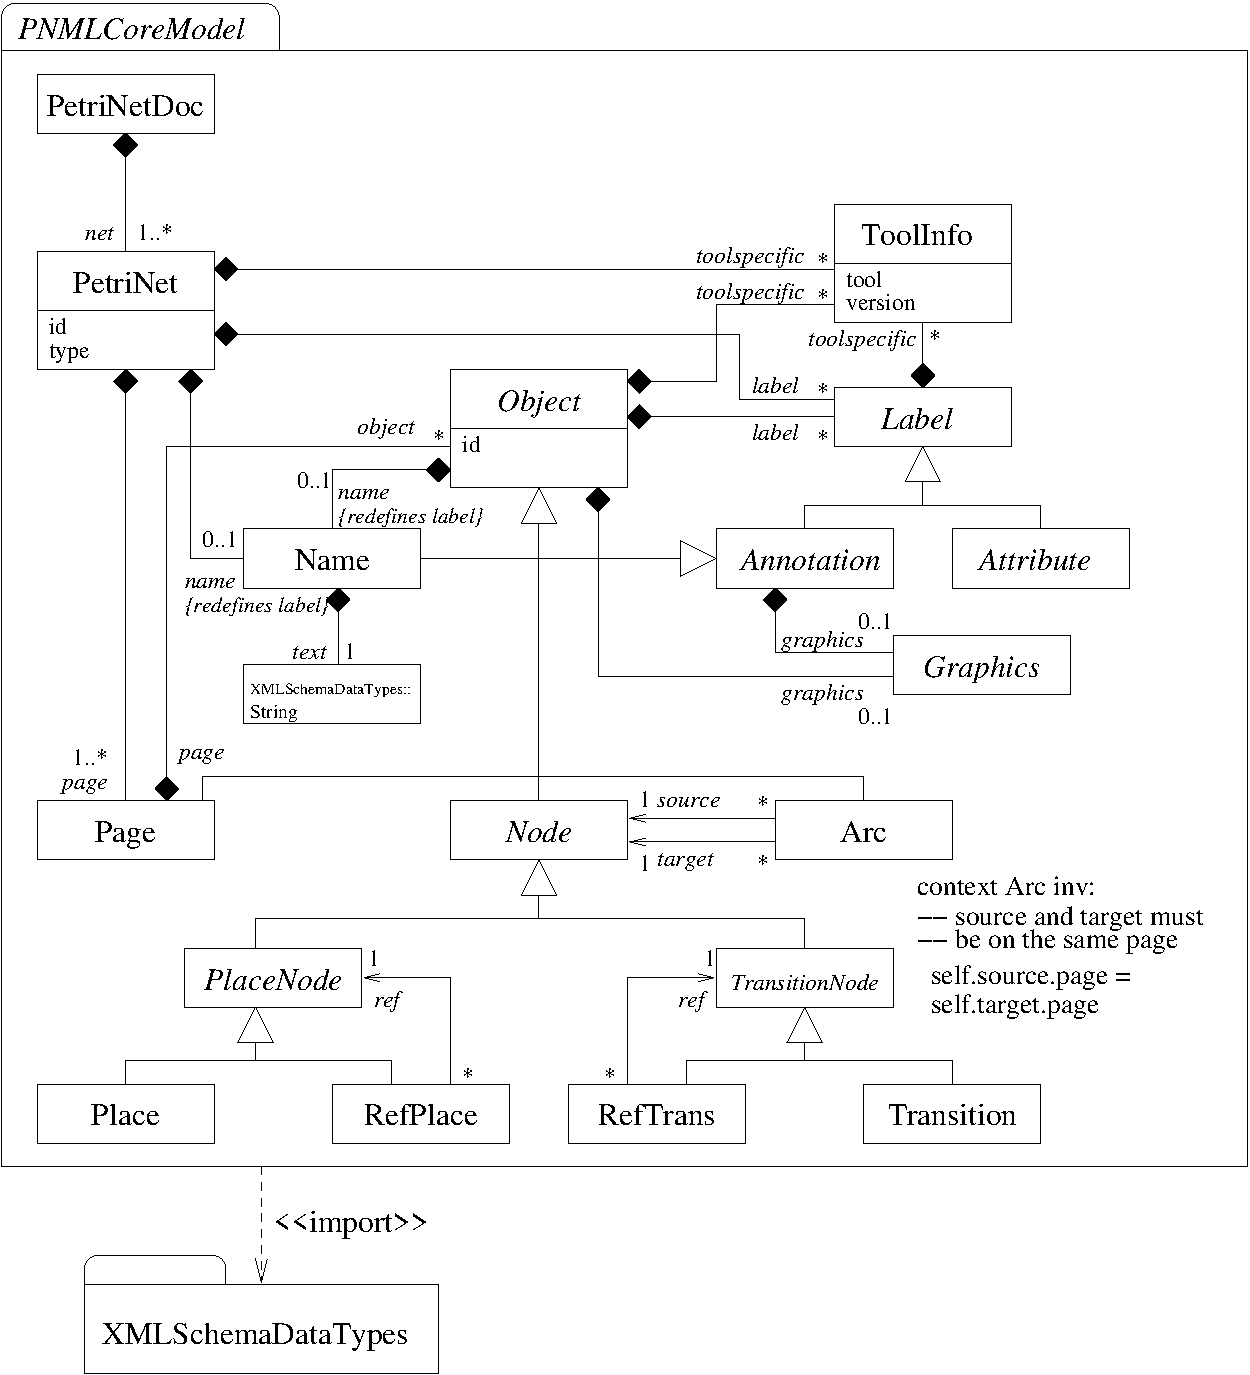
\includegraphics[scale=.58]{PNML_MetaModel}}
  \caption{The PNML core model of
    ISO/IEC~15909-2:2011 \cite{ISO-IEC:15909-2-2011}}
  \label{fig:MetaModel}%
  \index{PNML core model|DEF}
\end{figure}

Note that there is only one concrete type of label defined in the PNML core
model itself, which is the \emph{name} of an element.%
  \index{Petri net!Name|DEF}
All the other possible labels are defined in
separate Petri net type definitions, which are discussed in
Sect.~\ref{subsec:PNTD}.

In addition to the concepts and relations between them, the PNML core model
states also some restrictions on the structure of PNML models. For example,
there is a \emph{constraint}%
  \index{Constraint}
stating that arcs can connect only nodes that
are on the same page. This constraint if formulated as an \emph{OCL constraint}
in Fig.~\ref{fig:MetaModel}.
Note, however,
that there is no constraint in the PNML core model, which states that arcs must
run between a place and a transition or the other way round. The reason 
for not having such a constraint in the PNML core model is that there are
some kinds of Petri nets that would allow arcs between places or between 
transitions. This is why these kind of restrictions would be part of a
Petri net type definition.

Note also that the PNML core model does not specify concrete tool specific
extensions. It is up to a tool to define what it needs. But, any tool must be
able to read  -- and later write -- any tool specific extension; their contents
however, can be ignored.%
  \index{PNML core model|)}

\subsection{Petri net type definitions}
\label{subsec:PNTD}
\index{PNTD|(DEF}
As stated above, it is the purpose of a  \emph{Petri net type definition} to
define which labels are possible in a specific kind of Petri net, and also
to define some additional restrictions on the legal connections. Here,
we explain the idea of a Petri net type definition by the help of a simple
example: the definition of \emph{Place/Transition-Systems} (\emph{P/T-Systems}
in short).%
  \index{P/T-system|DEF}

The two additional kinds of labels for Place/Transition-Systems are the initial
marking for places, and the inscription for arcs.  The initial marking can be
any natural number (including 0) and the inscription for arcs can
be any positive number.  Figure~\ref{fig:PT-PNTD} shows the UML
model for these concepts and how they are related to the
concepts of the PNML core model.

\begin{figure}[hbt!!]
  \centerline{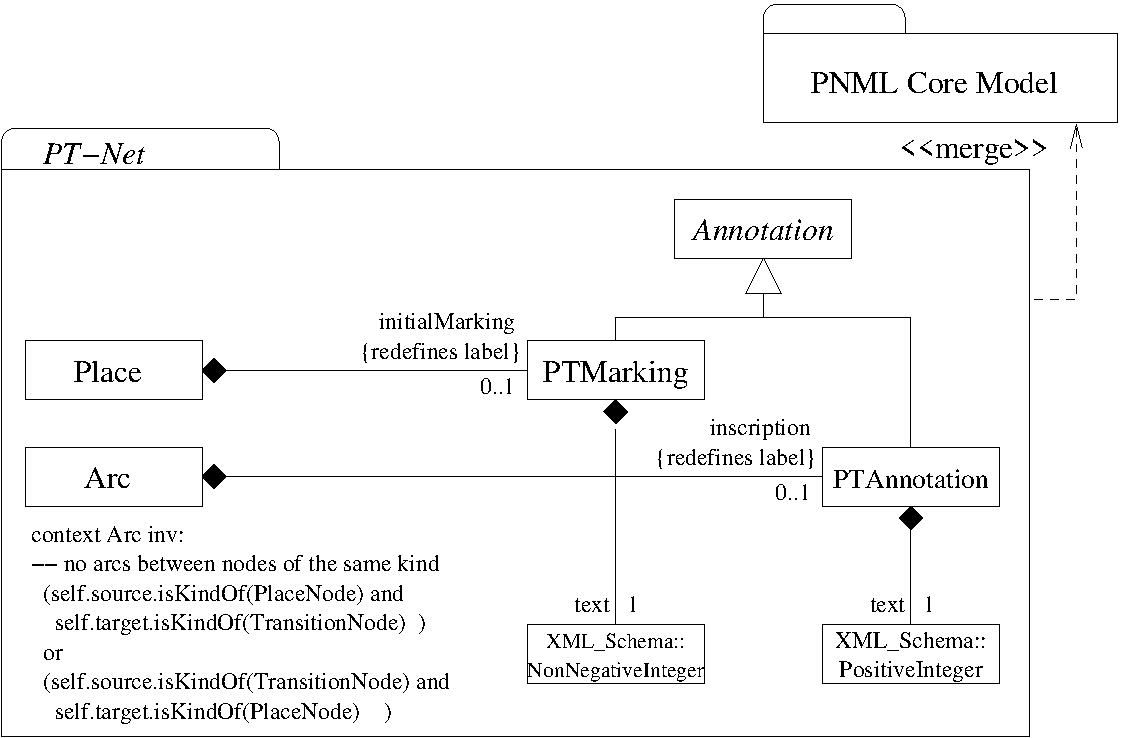
\includegraphics[scale=.60]{PT-PNTD}}
  \caption{The PNTD for PT-Nets}
  \label{fig:PT-PNTD}
\end{figure}

In Fig.~\ref{fig:PT-PNTD}, there is also one additional \emph{OCL constraint}.%
  \index{OCL constraint}
Without going into the details of OCL, this constraint states that
an arc must run from a place to a transition or from a transition to
a place. So, for P/T-Systems, it is no longer possible to connect places
with places or transitions with transitions.

A Petri net type definition, would typically also define how the new
concepts from Fig.~\ref{fig:PT-PNTD} would be mapped to XML. If not stated,
the ePNK will uses a default of how the new features are mapped to XML.
For the example above, this default mapping is good enough (and actually
compatible with ISO/IEC~15909-2).%
  \index{PNTD|)}

\subsection{Mapping to XML}
\label{subsec:XML-Mappings}
\index{PNML!XML format|(DEF}
As mentioned above, the PNML core model together with the model
for a Petri net type definition, define the concepts of a specific
kind of Petri net and how they can be connected. Therefore, these
models are the centerpiece of PNML. Still, PNML is an XML transfer
format for Petri nets. So, PNML defines how these concepts are saved or
represented in XML.  This is achieved by mapping every concept or feature of the
UML models to some XML construct. 


\begin{figure}[htbp]
  \centering
  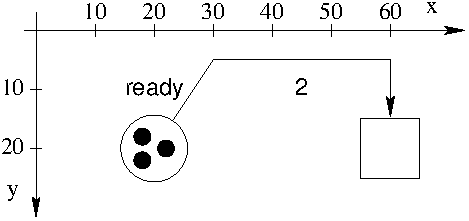
\includegraphics[scale=.5]{samplePTnet}
  \caption{A simple P/T-System}
  \label{fig:sample-net}
\end{figure} 

Here, we do not give these mappings, but rather 
show an example (for a detailed  discussion of the mappings,
see \cite{HKea09}). Figure~\ref{fig:sample-net} shows a simple example of a
P/T-System in its graphical representation (concrete syntax);
Listing~\ref{lst:sample-net} shows its representation in PNML's XML-syntax\footnote
  {We deleted some line-breaks to make this listing fit on a single page}.

\begin{figure}[p]
\lstinputlisting[language={[structured]PNML},keywordstyle=\underbar,label=lst:sample-net,%
caption={[PNML code of an example net]%
  PNML code of the example net in Fig.~\ref{fig:sample-net}}]%
  {samplePTnet.pnml}
\end{figure}

Note that the listing also shows an example of a tool specific extension:
the positions of the individual tokens in the place.%
  \index{PNML!XML format|)}%
  \index{PNML|)}

\section{ePNK: Objective}
\label{sec:Intro:Objective}

The main objective of the \emph{ePNK|DEF} was to build a tool that fully
supports the concepts of PNML, so that new Petri net types along with the mapping to
XML syntax can be easily plugged into this tool -- and to provide all the Petri
net type definitions for the types defined in ISO/IEC~15909-2:2011.

As soon as such a new Petri net type definition is plugged in, it
should be possible to load and save Petri net documents that contain
nets of these types. Moreover, there should be a graphical editor
that allows us to edit Petri nets of any plugged in Petri net type;
and the editor should be fully aware of all the features (annotations and
attributes) and the additional constraints of the plugged-in Petri net types.

For tool developers, the ePNK should provide an API to easily load and access
Petri nets from PNML files, to manipulate them, and to save them. Moreover, it
should be easy to plug in new functionality and \emph{applications}%
  \index{ePNK!Application}
for analysing Petri nets and for visualizing the results, and for manipulating
Petri nets or transforming them to other models or to code.

\section{How to read this manual}
\label{sec:Intro:Read}

In this manual, we will explain the features of the ePNK in more
detail. 

On the one-hand side, this manual covers the parts relevant for the
``end user'' who just wants to load, save and edit Petri nets of
existing types and use some existing or plugged in functionality
of the ePNK. In the rest of this manual, we call these ``end users'' just 
\emph{users}.%
  \index{ePNK!User|DEF}
All the information relevant for users of the ePNK
  can be found in Chapter~\ref{chap:users-guide}.


On the other-hand side, this manual covers the information relevant for
\emph{developers}%
  \index{ePNK!Developer|DEF} 
who are interested in using the ePNK for their
purposes: extending it by defining new Petri net types and their graphical
appearance, by defining new tool specific extensions, or by implementing
new functionality and applications. Chapter~\ref{chap:developers-guide} provides
the information relevant for developers who want to extend the ePNK.

Chapter~\ref{chap:tutorial} is a tutorial, which discusses the concepts
and the major steps of defining new Petri net types, their graphical
appearance, and a simple simulator application on top of it. The tutorial
goes into all the technical details, and is written in such a way that
it can be read independently from Chapter~\ref{chap:developers-guide}.

Chapter~\ref{chap:install} discusses the installation of Eclipse and
the ePNK as well as the major changes of version~1.2 of the ePNK 
with respect to version~1.0.

% In some future version of this manual, there will also be a part
% that discusses the architecture, the design, and some of the used technologies
% (and their  problems). These parts might be interesting for developers, but
% actually addresses people interested in model-based software development
% technologies that are used (and extended) in this project: EMF, GMF, Xtext,
% ExtendedMetaData, EMF Validation, and OCL. For now, we conclude this manual
% with Chapter~\ref{chap:inside}, which gives a brief experience report on the
% implementation of the ePNK and an overview of features of the ePNK that
% might be implemented in the future.

% During the development of the ePNK, we came across some problems and issues of
% PNML or ISO/IEC~15909-2. Chapter~\ref{chap:pnml-suggestions} will list and
% discuss these issues and make some suggestions for improving future versions
% of PNML or the definition of some specific Petri net types.
% Chapter~\ref{chap:pnml-suggestions} is mostly addressed to people interested
% in the standardisation process of ISO/IEC~15909 -- mostly concerning Parts~2
% and~3.
  